%\VignetteIndexEntry{Introduction to the GSqwsr package}
%\VignetteEngine{knitr::knitr}
%\VignetteDepends{}
%\VignetteSuggests{xtable}
%\VignettePackage{GSqwsr}

\documentclass[a4paper,11pt]{article}\usepackage[]{graphicx}\usepackage[]{color}
%% maxwidth is the original width if it is less than linewidth
%% otherwise use linewidth (to make sure the graphics do not exceed the margin)
\makeatletter
\def\maxwidth{ %
  \ifdim\Gin@nat@width>\linewidth
    \linewidth
  \else
    \Gin@nat@width
  \fi
}
\makeatother

\definecolor{fgcolor}{rgb}{0.345, 0.345, 0.345}
\newcommand{\hlnum}[1]{\textcolor[rgb]{0.686,0.059,0.569}{#1}}%
\newcommand{\hlstr}[1]{\textcolor[rgb]{0.192,0.494,0.8}{#1}}%
\newcommand{\hlcom}[1]{\textcolor[rgb]{0.678,0.584,0.686}{\textit{#1}}}%
\newcommand{\hlopt}[1]{\textcolor[rgb]{0,0,0}{#1}}%
\newcommand{\hlstd}[1]{\textcolor[rgb]{0.345,0.345,0.345}{#1}}%
\newcommand{\hlkwa}[1]{\textcolor[rgb]{0.161,0.373,0.58}{\textbf{#1}}}%
\newcommand{\hlkwb}[1]{\textcolor[rgb]{0.69,0.353,0.396}{#1}}%
\newcommand{\hlkwc}[1]{\textcolor[rgb]{0.333,0.667,0.333}{#1}}%
\newcommand{\hlkwd}[1]{\textcolor[rgb]{0.737,0.353,0.396}{\textbf{#1}}}%

\usepackage{framed}
\makeatletter
\newenvironment{kframe}{%
 \def\at@end@of@kframe{}%
 \ifinner\ifhmode%
  \def\at@end@of@kframe{\end{minipage}}%
  \begin{minipage}{\columnwidth}%
 \fi\fi%
 \def\FrameCommand##1{\hskip\@totalleftmargin \hskip-\fboxsep
 \colorbox{shadecolor}{##1}\hskip-\fboxsep
     % There is no \\@totalrightmargin, so:
     \hskip-\linewidth \hskip-\@totalleftmargin \hskip\columnwidth}%
 \MakeFramed {\advance\hsize-\width
   \@totalleftmargin\z@ \linewidth\hsize
   \@setminipage}}%
 {\par\unskip\endMakeFramed%
 \at@end@of@kframe}
\makeatother

\definecolor{shadecolor}{rgb}{.97, .97, .97}
\definecolor{messagecolor}{rgb}{0, 0, 0}
\definecolor{warningcolor}{rgb}{1, 0, 1}
\definecolor{errorcolor}{rgb}{1, 0, 0}
\newenvironment{knitrout}{}{} % an empty environment to be redefined in TeX

\usepackage{alltt}

\usepackage{amsmath}
\usepackage{times}
\usepackage{hyperref}
\usepackage[numbers, round]{natbib}
\usepackage[american]{babel}
\usepackage{authblk}
\usepackage{subfig}
\usepackage{placeins}
\usepackage{footnote}
\usepackage{tabularx}
\usepackage{threeparttable}
\usepackage{parskip}

\usepackage{csquotes}
\usepackage{setspace}

% \doublespacing

\renewcommand{\topfraction}{0.85}
\renewcommand{\textfraction}{0.1}
\usepackage{graphicx}


\usepackage{mathptmx}% Times Roman font
\usepackage[scaled=.90]{helvet}% Helvetica, served as a model for arial

% \usepackage{indentfirst}
% \setlength\parindent{20pt}
\setlength{\parskip}{0pt}

\usepackage{courier}

\usepackage{titlesec}
\usepackage{titletoc}

\titleformat{\section}
  {\normalfont\sffamily\bfseries\LARGE}
  {\thesection}{0.5em}{}
\titleformat{\subsection}
  {\normalfont\sffamily\bfseries\Large}
  {\thesubsection}{0.5em}{}
\titleformat{\subsubsection}
  {\normalfont\sffamily\large}
  {\thesubsubsection}{0.5em}{}
  
\titlecontents{section}
[2em]                 % adjust left margin
{\sffamily}             % font formatting
{\contentslabel{2.3em}} % section label and offset
{\hspace*{-2.3em}}
{\titlerule*[0.25pc]{.}\contentspage}
  
\titlecontents{subsection}
[4.6em]                 % adjust left margin
{\sffamily}             % font formatting
{\contentslabel{2.3em}} % section label and offset
{\hspace*{-2.3em}}
{\titlerule*[0.25pc]{.}\contentspage}
  
\titlecontents{subsubsection}
[6.9em]                 % adjust left margin
{\sffamily}             % font formatting
{\contentslabel{2.3em}} % section label and offset
{\hspace*{-2.3em}}
{\titlerule*[0.25pc]{.}\contentspage}

\titlecontents{table}
[0em]                 % adjust left margin
{\sffamily}             % font formatting
{Table\hspace*{2em} \contentslabel {2em}} % section label and offset
{\hspace*{4em}}
{\titlerule*[0.25pc]{.}\contentspage}

\titlecontents{figure}
[0em]                 % adjust left margin
{\sffamily}             % font formatting
{Figure\hspace*{2em} \contentslabel {2em}} % section label and offset
{\hspace*{4em}}
{\titlerule*[0.25pc]{.}\contentspage}

%Italisize and change font of urls:
\urlstyle{sf}
\renewcommand\UrlFont\itshape

\usepackage{caption}
\captionsetup{
  font={sf},
  labelfont={bf,sf},
  labelsep=period,
  justification=justified,
  singlelinecheck=false
}



\textwidth=6.2in
\textheight=8.5in
\parskip=.3cm
\oddsidemargin=.1in
\evensidemargin=.1in
\headheight=-.3in


%------------------------------------------------------------
% newcommand
%------------------------------------------------------------
\newcommand{\scscst}{\scriptscriptstyle}
\newcommand{\scst}{\scriptstyle}
\newcommand{\Robject}[1]{{\texttt{#1}}}
\newcommand{\Rfunction}[1]{{\texttt{#1}}}
\newcommand{\Rclass}[1]{\textit{#1}}
\newcommand{\Rpackage}[1]{\textit{#1}}
\newcommand{\Rexpression}[1]{\texttt{#1}}
\newcommand{\Rmethod}[1]{{\texttt{#1}}}
\newcommand{\Rfunarg}[1]{{\texttt{#1}}}
\IfFileExists{upquote.sty}{\usepackage{upquote}}{}
\begin{document}



\renewenvironment{knitrout}{\begin{singlespace}}{\end{singlespace}}
\renewcommand*\listfigurename{Figures}

\renewcommand*\listtablename{Tables}


%------------------------------------------------------------
\title{The dataRetrieval R package}
%------------------------------------------------------------
\author[1]{Laura De Cicco}
\author[1]{Steve Corsi}
\affil[1]{United States Geological Survey}




\noindent{\huge\textsf{\textbf{The GSqwsr R package: Water Quality Surrogate Regressions}}}

\noindent\textsf{By Laura De Cicco and Steve Corsi}

\noindent\textsf{\today}

% \maketitle
% 
% \newpage 

\tableofcontents
\listoffigures
\listoftables

\newpage


%------------------------------------------------------------
\section{Introduction to GSqwsr package}
%------------------------------------------------------------ 
The GSqwsr (USGS water quality surrogate regressions) package was designed to simplify the process of gathering water quality sample data and unit surrogate data, running a stepwise regression using the USGSwsQW censReg regression function, and analyzing those results. This vignette will first show a general overview workflow  (\ref{sec:workflow}), then a more detailed description of the workflow with working examples (\ref{sec:details}).

%------------------------------------------------------------
\section{General Workflow}
\label{sec:workflow}
%------------------------------------------------------------ 

\begin{knitrout}
\definecolor{shadecolor}{rgb}{0.969, 0.969, 0.969}\color{fgcolor}\begin{kframe}
\begin{alltt}
\hlkwd{library}\hlstd{(}\hlstr{"GSqwsr"}\hlstd{)}

\hlcom{#Sample data included with package:}
\hlstd{DTComplete} \hlkwb{<-} \hlstd{StLouisDT}
\hlstd{UV} \hlkwb{<-} \hlstd{StLouisUV}
\hlstd{QWcodes} \hlkwb{<-} \hlstd{StLouisQWcodes}
\hlstd{siteINFO} \hlkwb{<-} \hlstd{StLouisInfo}

\hlstd{investigateResponse} \hlkwb{<-} \hlstr{"Ammonia.N"}
\hlstd{transformResponse} \hlkwb{<-} \hlstr{"lognormal"}

\hlstd{DT} \hlkwb{<-} \hlstd{DTComplete[}\hlkwd{c}\hlstd{(investigateResponse,}
                   \hlkwd{getPredictVariables}\hlstd{(}\hlkwd{names}\hlstd{(UV)),}
                   \hlstr{"decYear"}\hlstd{,}\hlstr{"sinDY"}\hlstd{,}\hlstr{"cosDY"}\hlstd{,}\hlstr{"datetime"}\hlstd{)]}
\hlstd{DT} \hlkwb{<-} \hlkwd{na.omit}\hlstd{(DT)}

\hlstd{predictVariables} \hlkwb{<-} \hlkwd{names}\hlstd{(DT)[}\hlopt{-}\hlkwd{which}\hlstd{(}\hlkwd{names}\hlstd{(DT)}
                  \hlopt \hlkwd{c}\hlstd{(investigateResponse,}\hlstr{"datetime"}\hlstd{,}\hlstr{"decYear"}\hlstd{))]}


\hlcom{#Check predictor variables}
\hlkwd{predictVariableScatterPlots}\hlstd{(DT,investigateResponse)}

\hlcom{# Create 'kitchen sink' formula:}
\hlstd{kitchenSink} \hlkwb{<-} \hlkwd{createFullFormula}\hlstd{(DT,investigateResponse)}

\hlcom{#Run stepwise regression with "kitchen sink" as upper bound:}
\hlstd{returnPrelim} \hlkwb{<-} \hlkwd{prelimModelDev}\hlstd{(DT,investigateResponse,kitchenSink,}
                               \hlstr{"BIC"}\hlstd{,} \hlcom{#Other option is "AIC"}
                               \hlstd{transformResponse)}

\hlstd{steps} \hlkwb{<-} \hlstd{returnPrelim}\hlopt{$}\hlstd{steps}
\hlstd{modelResult} \hlkwb{<-} \hlstd{returnPrelim}\hlopt{$}\hlstd{modelInformation}
\hlstd{modelReturn} \hlkwb{<-} \hlstd{returnPrelim}\hlopt{$}\hlstd{DT.mod}

\hlcom{# Analyze steps found:}
\hlkwd{plotSteps}\hlstd{(steps,DT,transformResponse)}
\hlkwd{analyzeSteps}\hlstd{(steps, investigateResponse,siteINFO)}

\hlcom{# Analyze model produced from stepwise regression:}
\hlkwd{resultPlots}\hlstd{(DT,modelReturn,siteINFO)}
\hlkwd{resultResidPlots}\hlstd{(DT,modelReturn,siteINFO)}

\hlcom{# Create prediction plots}
\hlkwd{predictionPlot}\hlstd{(UV,DT,modelReturn,}\hlkwc{siteINFO}\hlstd{=siteINFO)}
\end{alltt}
\end{kframe}
\end{knitrout}


%------------------------------------------------------------
\section{Workflow Details}
\label{sec:details}
%------------------------------------------------------------
In this section, we will step through the basic workflow.

%------------------------------------------------------------
\subsection{Data Retrieval}
%------------------------------------------------------------
Data retrieval is currently supported by web service calls to the National Water Information Service (NWIS). The first step is to get the discrete sample data that the regressions are modeling. In this example, we will look at the St Louis River at Scanlon (USGS site ID 04024000). If we don't know the sample data that is available, we can use the whatQW function to discover that information. 

\begin{knitrout}
\definecolor{shadecolor}{rgb}{0.969, 0.969, 0.969}\color{fgcolor}\begin{kframe}
\begin{alltt}
\hlkwd{library}\hlstd{(GSqwsr)}
\end{alltt}
\end{kframe}
\end{knitrout}




\begin{knitrout}
\definecolor{shadecolor}{rgb}{0.969, 0.969, 0.969}\color{fgcolor}\begin{kframe}
\begin{alltt}
\hlstd{site} \hlkwb{<-} \hlstr{"04024000"}
\hlstd{QWcodes} \hlkwb{<-} \hlkwd{whatQW}\hlstd{(site,} \hlkwc{minCount}\hlstd{=}\hlnum{20}\hlstd{)}
\hlkwd{head}\hlstd{(QWcodes)}
\end{alltt}
\begin{verbatim}
  parameter_cd  startDate    endDate count service
1        00010 1964-10-28 2014-09-15   276      qw
2        00020 1974-10-30 2014-09-15   165      qw
3        00025 1981-10-20 2014-09-15   145      qw
4        00041 2010-10-07 2013-06-11    55      qw
5        00055 2010-10-07 2013-04-27    35      qw
6        00061 1960-07-28 2014-09-15   315      qw
\end{verbatim}
\end{kframe}
\end{knitrout}

Most likely, there will be a known set of parameters that are to be modeled. If the parameter codes for these analytes are known, the data from NWIS can be accessed directly with the function importNWISqw. The following example shows the process, and then lists the column names returned in the QW dataframe.


\begin{knitrout}
\definecolor{shadecolor}{rgb}{0.969, 0.969, 0.969}\color{fgcolor}\begin{kframe}
\begin{alltt}
\hlstd{pCodeQW} \hlkwb{<-} \hlkwd{c}\hlstd{(}\hlstr{"00608"}\hlstd{,}\hlstr{"00613"}\hlstd{,}\hlstr{"00618"}\hlstd{)}
\hlstd{startDate} \hlkwb{<-} \hlstr{"2011-04-22"}
\hlstd{endDate} \hlkwb{<-} \hlstr{""}
\hlstd{QW} \hlkwb{<-} \hlkwd{importNWISqw}\hlstd{(site,} \hlkwc{params}\hlstd{=pCodeQW,}
                   \hlkwc{begin.date}\hlstd{=startDate,} \hlkwc{end.date}\hlstd{=endDate)}
\end{alltt}
\end{kframe}
\end{knitrout}



\begin{knitrout}
\definecolor{shadecolor}{rgb}{0.969, 0.969, 0.969}\color{fgcolor}\begin{kframe}
\begin{alltt}
\hlkwd{names}\hlstd{(QW)}
\end{alltt}
\begin{verbatim}
 [1] "site_no"              "sample_dt"           
 [3] "sample_tm"            "tzone_cd"            
 [5] "medium_cd"            "Ammonia.N"           
 [7] "Nitrite.N"            "Nitrate.N"           
 [9] "NO2PlusNO3.N"         "Phosphorus_WW.P"     
[11] "OrthoPhosphate.P"     "Chloride"            
[13] "NitrogenTotal_WW.sum" "SuspSed"             
[15] "datetime"            
\end{verbatim}
\end{kframe}
\end{knitrout}


This brings the data in automatically as a \texttt{"qw"} object. This means that censoring information is embedded within each data point. If any processing needs to be done to the data, it might be easier to import the raw data first, then convert to \texttt{"qw"} objects with the makeQWObjects function.

\begin{knitrout}
\definecolor{shadecolor}{rgb}{0.969, 0.969, 0.969}\color{fgcolor}\begin{kframe}
\begin{alltt}
\hlstd{QWRaw} \hlkwb{<-} \hlkwd{retrieveNWISqwData}\hlstd{(site,pCodeQW,startDate,}
                            \hlstd{endDate,}\hlkwc{expanded}\hlstd{=}\hlnum{TRUE}\hlstd{)}
\hlstd{QW} \hlkwb{<-} \hlkwd{makeQWObjects}\hlstd{(QWRaw)}
\end{alltt}
\end{kframe}
\end{knitrout}

Next, the unit value data that will be used as surrogates for the analytes should be retrieved. If the parameters are not known, they can be discovered using the getDataAvailability function, filtering just the \enquote{uv} (unit value) data:

\begin{knitrout}
\definecolor{shadecolor}{rgb}{0.969, 0.969, 0.969}\color{fgcolor}\begin{kframe}
\begin{alltt}
\hlkwd{library}\hlstd{(dataRetrieval)}
\hlstd{UVcodes} \hlkwb{<-} \hlkwd{getNWISDataAvailability}\hlstd{(site)}
\hlstd{UVcodes} \hlkwb{<-} \hlstd{UVcodes[UVcodes}\hlopt{$}\hlstd{service} \hlopt{==} \hlstr{"uv"}\hlstd{,]}
\hlkwd{names}\hlstd{(UVcodes)}
\end{alltt}
\begin{verbatim}
 [1] "parameter_cd"       "site_no"           
 [3] "statCd"             "startDate"         
 [5] "endDate"            "count"             
 [7] "service"            "parameter_group_nm"
 [9] "parameter_nm"       "casrn"             
[11] "srsname"            "parameter_units"   
\end{verbatim}
\begin{alltt}
\hlstd{UVcodes}\hlopt{$}\hlstd{parameter_cd}
\end{alltt}
\begin{verbatim}
[1] "00010" "00021" "00060" "00065" "00095" "00300" "00301"
[8] "00400" "63680"
\end{verbatim}
\end{kframe}
\end{knitrout}

Finally, the unit value data can be retrieved with the getMultipleUV function. Because of the potentially large amount of data being returned, the web service call is automatically split into individual parameter codes.

\begin{knitrout}
\definecolor{shadecolor}{rgb}{0.969, 0.969, 0.969}\color{fgcolor}\begin{kframe}
\begin{alltt}
\hlstd{UVpCodes} \hlkwb{<-} \hlkwd{c}\hlstd{(}\hlstr{"00010"}\hlstd{,}\hlstr{"00060"}\hlstd{,}\hlstr{"00095"}\hlstd{,}\hlstr{"00300"}\hlstd{,}\hlstr{"00400"}\hlstd{,}\hlstr{"63680"}\hlstd{)}
\hlstd{UV} \hlkwb{<-} \hlkwd{getMultipleUV}\hlstd{(site, startDate, endDate, UVpCodes)}
\end{alltt}
\end{kframe}
\end{knitrout}



\begin{knitrout}
\definecolor{shadecolor}{rgb}{0.969, 0.969, 0.969}\color{fgcolor}\begin{kframe}
\begin{alltt}
\hlkwd{names}\hlstd{(UV)}
\end{alltt}
\begin{verbatim}
 [1] "agency_cd"   "site_no"     "datetime"    "tz_cd"      
 [5] "Wtemp"       "Wtemp_cd"    "Flow"        "Flow_cd"    
 [9] "SpecCond"    "SpecCond_cd" "DO"          "DO_cd"      
[13] "pH"          "pH_cd"       "Turb"        "Turb_cd"    
\end{verbatim}
\end{kframe}
\end{knitrout}


%------------------------------------------------------------
\subsection{Data Merging}
%------------------------------------------------------------
We now need to merge the sample and continuous data into one dataframe. This is accomplished using the mergeDatasets function. Both QW and UV dataframes need a column called `datetime' that has the date and time in an POSIXct object. This may need to be done as shown below.


\begin{knitrout}
\definecolor{shadecolor}{rgb}{0.969, 0.969, 0.969}\color{fgcolor}\begin{kframe}
\begin{alltt}
\hlstd{QW}\hlopt{$}\hlstd{datetime} \hlkwb{<-} \hlkwd{as.POSIXct}\hlstd{(}\hlkwd{paste}\hlstd{(QW}\hlopt{$}\hlstd{sample_dt,}\hlstr{" "}\hlstd{,QW}\hlopt{$}\hlstd{sample_tm,} \hlstr{":00"}\hlstd{,}\hlkwc{sep}\hlstd{=}\hlstr{""}\hlstd{))}

\hlcom{# Make sure they are in consistant time zones:}
\hlstd{QW}\hlopt{$}\hlstd{datetime} \hlkwb{<-} \hlkwd{setTZ}\hlstd{(QW}\hlopt{$}\hlstd{datetime, QW}\hlopt{$}\hlstd{tzone_cd)}
\hlstd{UV}\hlopt{$}\hlstd{datetime} \hlkwb{<-} \hlkwd{setTZ}\hlstd{(UV}\hlopt{$}\hlstd{datetime, UV}\hlopt{$}\hlstd{tz_cd)}

\hlstd{mergeReturn} \hlkwb{<-} \hlkwd{mergeDatasets}\hlstd{(QW, UV, QWcodes)}
\hlstd{DTComplete} \hlkwb{<-} \hlstd{mergeReturn}\hlopt{$}\hlstd{DTComplete}
\hlstd{QWcodes} \hlkwb{<-} \hlstd{mergeReturn}\hlopt{$}\hlstd{QWcodes}
\end{alltt}
\end{kframe}
\end{knitrout}

The dataframe DTComplete contains a column of each of the discrete samples, and a column of the nearest (temporally) unit value data. The function mergeDatasets has an argument called `max.diff'. The default is set to `2 hours', meaning that if the sample and continuous data timestamps do not match, the merge will take the closest continuous data within 2 hours. This value can be changed, see ?mergeNearest for more options.

%------------------------------------------------------------
\subsection{Data Investigation}
%------------------------------------------------------------

%------------------------------------------------------------
\subsubsection{Narrow down investigation}
%------------------------------------------------------------


We now want to narrow our investigation down to one analyte. Let us look at nitrate. First we will want a dataframe DT with just nitrate and the unit values. We will call these the `prediction values' because they will eventually be used to predict nitrate.

\begin{knitrout}
\definecolor{shadecolor}{rgb}{0.969, 0.969, 0.969}\color{fgcolor}\begin{kframe}
\begin{alltt}
\hlstd{investigateResponse} \hlkwb{<-} \hlstr{"Nitrate.N"}
\hlstd{predictionVariables} \hlkwb{<-} \hlkwd{getPredictVariables}\hlstd{(}\hlkwd{names}\hlstd{(UV))}

\hlstd{DT} \hlkwb{<-} \hlstd{DTComplete[}\hlkwd{c}\hlstd{(investigateResponse,}
                   \hlstd{predictionVariables,}
                   \hlstr{"decYear"}\hlstd{,}\hlstr{"sinDY"}\hlstd{,}\hlstr{"cosDY"}\hlstd{,}\hlstr{"datetime"}\hlstd{)]}

\hlkwd{names}\hlstd{(DT)}
\end{alltt}
\begin{verbatim}
 [1] "Nitrate.N" "Wtemp"     "Flow"      "SpecCond" 
 [5] "DO"        "pH"        "Turb"      "decYear"  
 [9] "sinDY"     "cosDY"     "datetime" 
\end{verbatim}
\end{kframe}
\end{knitrout}

For the regression, there can be no NA values in any of the columns. There are many ways in R to deal with this requirement. The easiest way to do it is remove any row that has any NA. This can be done as follows:

\begin{knitrout}
\definecolor{shadecolor}{rgb}{0.969, 0.969, 0.969}\color{fgcolor}\begin{kframe}
\begin{alltt}
\hlstd{DT} \hlkwb{<-} \hlkwd{na.omit}\hlstd{(DT)}
\end{alltt}
\end{kframe}
\end{knitrout}

There may be other situations where you want to remove a column that contains the majority of the missing data.

%------------------------------------------------------------
\subsubsection{Plot variables}
%------------------------------------------------------------
There are a few tools included in this package to explore the data before performing the regression.

\begin{knitrout}
\definecolor{shadecolor}{rgb}{0.969, 0.969, 0.969}\color{fgcolor}\begin{kframe}
\begin{alltt}
\hlkwd{plotQQTransforms}\hlstd{(DT,investigateResponse)}
\end{alltt}
\end{kframe}\begin{figure}[]

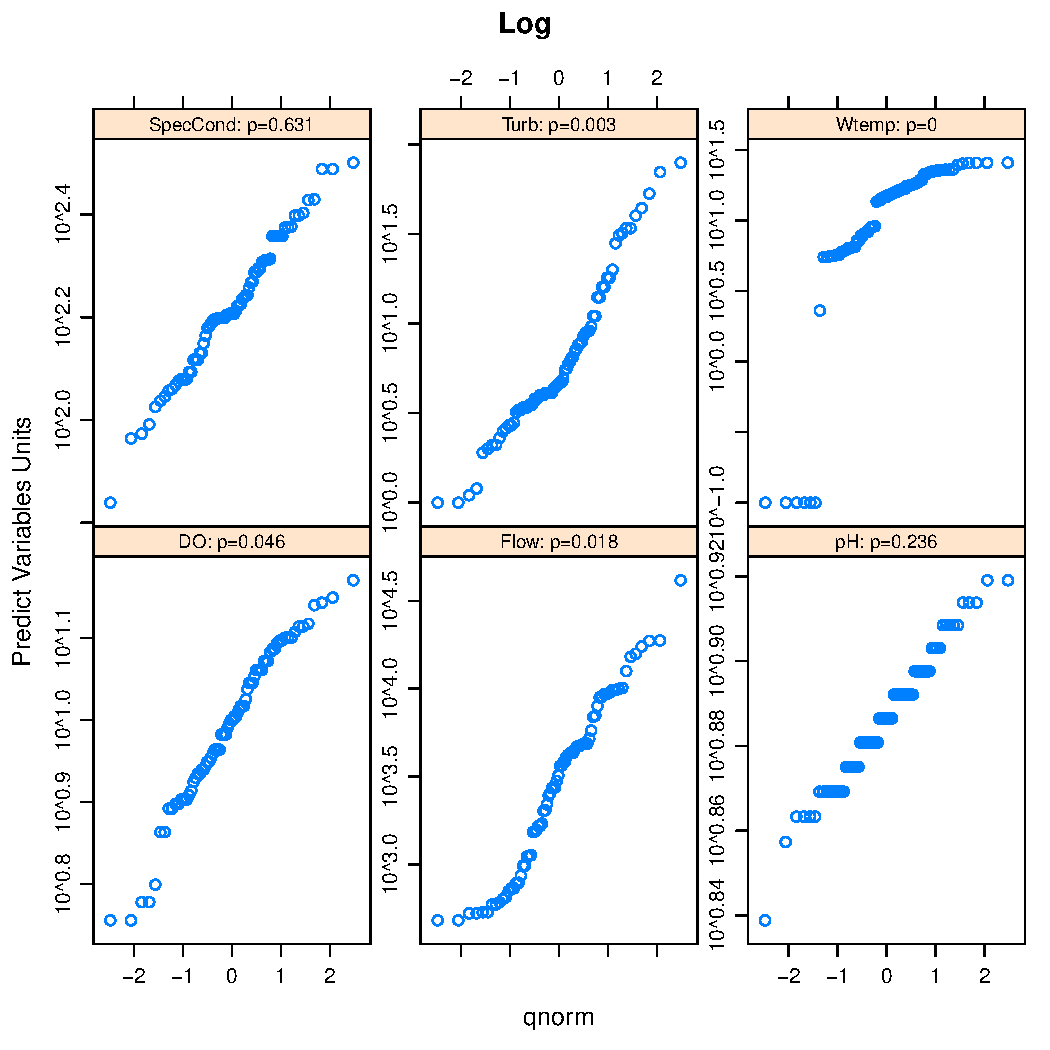
\includegraphics[width=\maxwidth]{figure/plotQQTransforms1} \caption[plotQQTransforms]{plotQQTransforms\label{fig:plotQQTransforms1}}
\end{figure}

\begin{figure}[]

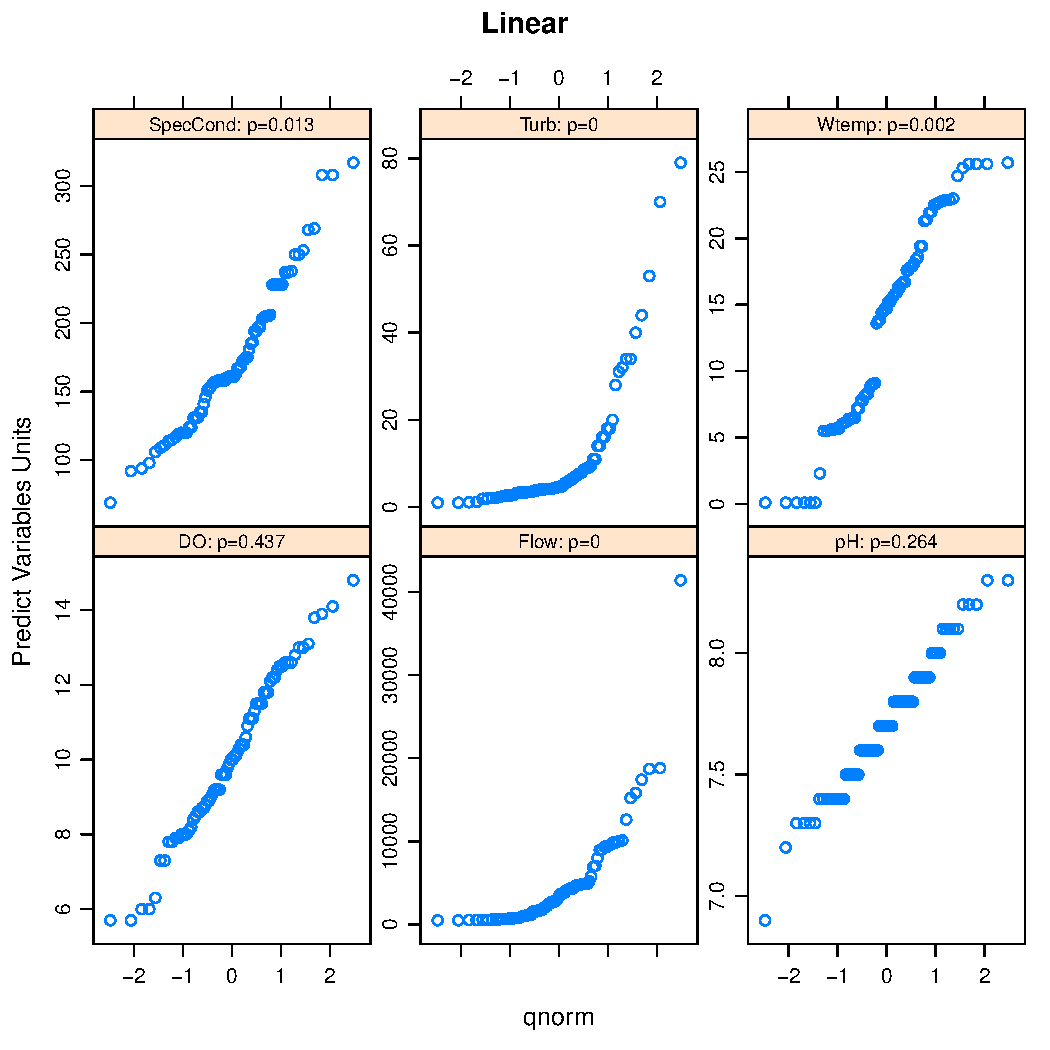
\includegraphics[width=\maxwidth]{figure/plotQQTransforms2} \caption[plotQQTransforms]{plotQQTransforms\label{fig:plotQQTransforms2}}
\end{figure}


\end{knitrout}


\begin{knitrout}
\definecolor{shadecolor}{rgb}{0.969, 0.969, 0.969}\color{fgcolor}\begin{kframe}
\begin{alltt}
\hlkwd{predictVariableScatterPlots}\hlstd{(DT,investigateResponse)}
\end{alltt}
\end{kframe}\begin{figure}[]

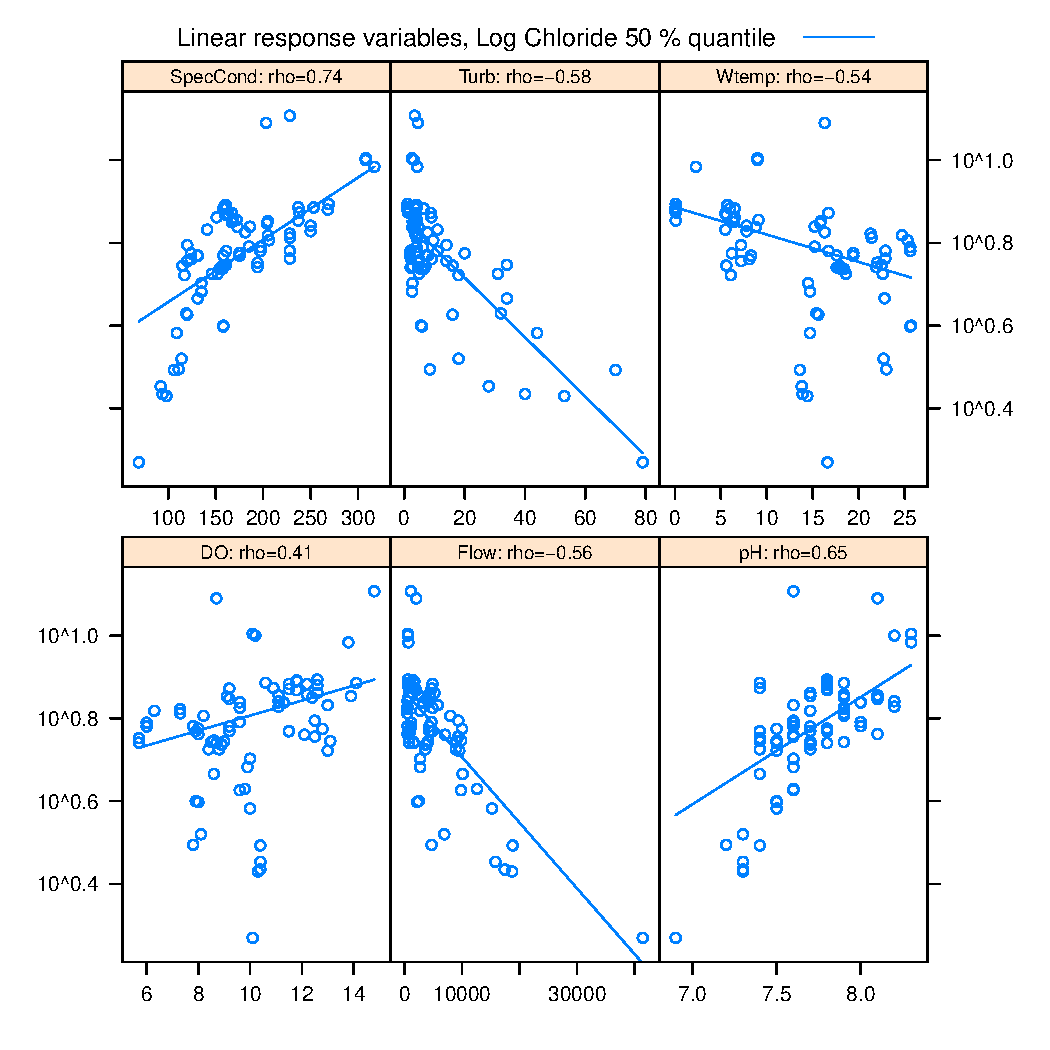
\includegraphics[width=\maxwidth]{figure/predictVariableScatterPlots1} \caption[predictVariableScatterPlots]{predictVariableScatterPlots\label{fig:predictVariableScatterPlots1}}
\end{figure}

\begin{figure}[]

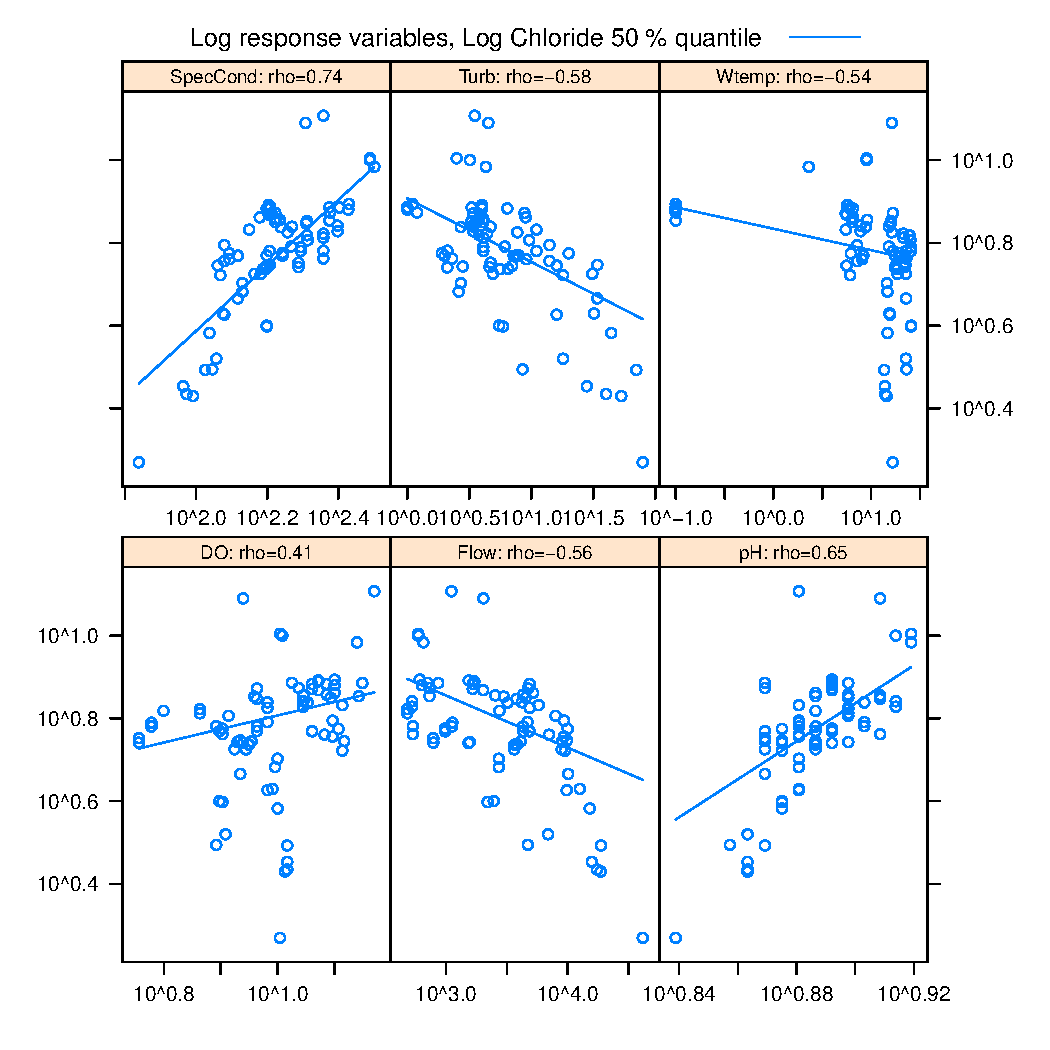
\includegraphics[width=\maxwidth]{figure/predictVariableScatterPlots2} \caption[predictVariableScatterPlots]{predictVariableScatterPlots\label{fig:predictVariableScatterPlots2}}
\end{figure}


\end{knitrout}

\FloatBarrier
%------------------------------------------------------------
\subsection{Stepwise Regression}
%------------------------------------------------------------
We are ready to perform a stepwise regression of the data to find the most significant variables to use in the model. This is accomplished with the prelimModelDev function. There are several inputs to this function. DT is the dataframe with all the predictor variables as well as the response we are investigating. We also need to define an upper bound for the stepwise regression to test. This is an equation with all the possible predictor variables, along with their transforms that we are interested in testing. If we want to use all possible variables, and all available transforms, we can use the equation createFullFormula (continuing with our Chloride example):

\begin{knitrout}
\definecolor{shadecolor}{rgb}{0.969, 0.969, 0.969}\color{fgcolor}\begin{kframe}
\begin{alltt}
\hlstd{upperBoundFormula} \hlkwb{<-} \hlkwd{createFullFormula}\hlstd{(DT,investigateResponse)}
\end{alltt}
\end{kframe}
\end{knitrout}

\begin{knitrout}
\definecolor{shadecolor}{rgb}{0.969, 0.969, 0.969}\color{fgcolor}\begin{kframe}
\begin{verbatim}
[1] "Wtemp + Flow + SpecCond + DO + pH + Turb + sinDY + cosDY + "
[1] "log(Flow) + log(SpecCond) + log(DO) + log(Turb)"
\end{verbatim}
\end{kframe}
\end{knitrout}

The function will check if any data in DT has less than or equal to zero values. If so, a log transform is not included.

Now to use the stepwise regression within the prelimModelDev function. In this function, the DT dataframe is required, the column name of the response variable (in this example, investigateResponse), and the upper bound formula. The user can then choose a value for k which can be `AIC' (akaike information criterion), `BIC' (Bayesian information criterion), or a value of the multiple of the number of degrees of freedom used for the penalty. BIC has a harsher penalty for overfitting the model, which is typically seen as a benefit. The default is BIC. Finally, transformResponse can either be `lognormal' or `normal', which will define the transformation of the response variable. 

Additionally, this function has an argument 'autoSinCos' which is a logical input. The default is set to TRUE, in this case - if the sine of decimal year (sinDY) is picked during the stepwise regression, the next step is forced to be cosDY. Likewise, if cosDY is picked, sinDY is forced on the next step. This feature can be turned off by setting autoSinCos to FALSE.


\begin{knitrout}
\definecolor{shadecolor}{rgb}{0.969, 0.969, 0.969}\color{fgcolor}\begin{kframe}
\begin{alltt}
\hlstd{transformResponse} \hlkwb{<-} \hlstr{"lognormal"}

\hlstd{returnPrelim} \hlkwb{<-} \hlkwd{prelimModelDev}\hlstd{(DT,}
                 \hlstd{investigateResponse,}
                 \hlstd{upperBoundFormula,}
                 \hlstr{"BIC"}\hlstd{,} \hlcom{#Other option is "AIC"}
                 \hlstd{transformResponse)}
\end{alltt}
\begin{verbatim}
Start:  AIC=182.3
Nitrate.N ~ 1

                Df AIC
+ sinDY          1 155
+ DO             1 174
+ Wtemp          1 175
+ log(DO)        1 177
+ pH             1 177
<none>             182
+ log(Flow)      1 184
+ SpecCond       1 184
+ cosDY          1 184
+ log(SpecCond)  1 185
+ log(Turb)      1 186
+ Turb           1 186
+ Flow           1 187

Step:  AIC=154.6
Nitrate.N ~ sinDY

                Df AIC
<none>             155
+ cosDY          1 156
+ pH             1 156
+ log(SpecCond)  1 156
+ SpecCond       1 157
+ Flow           1 158
+ log(Flow)      1 158
+ log(Turb)      1 159
+ log(DO)        1 159
+ Wtemp          1 159
+ Turb           1 159
+ DO             1 159
- sinDY          1 182
Start:  AIC=155.9
Nitrate.N ~ sinDY + cosDY

                Df AIC
+ pH             1 154
+ Wtemp          1 155
+ log(DO)        1 156
<none>             156
+ DO             1 159
+ log(SpecCond)  1 160
+ Flow           1 160
+ log(Turb)      1 160
+ SpecCond       1 160
+ Turb           1 160
+ log(Flow)      1 160

Step:  AIC=154.4
Nitrate.N ~ sinDY + cosDY + pH

                Df AIC
+ log(SpecCond)  1 143
+ SpecCond       1 151
+ Flow           1 152
+ Wtemp          1 154
+ log(DO)        1 154
<none>             154
- pH             1 156
+ log(Flow)      1 156
+ DO             1 157
+ Turb           1 157
+ log(Turb)      1 157

Step:  AIC=143.4
Nitrate.N ~ sinDY + cosDY + pH + log(SpecCond)

                Df AIC
+ Wtemp          1 139
+ SpecCond       1 141
<none>             143
+ log(DO)        1 145
+ DO             1 146
+ log(Turb)      1 147
+ log(Flow)      1 148
+ Turb           1 148
+ Flow           1 148
- log(SpecCond)  1 154
- pH             1 160

Step:  AIC=138.8
Nitrate.N ~ sinDY + cosDY + pH + log(SpecCond) + Wtemp

                Df AIC
+ log(Turb)      1 129
+ log(Flow)      1 135
+ DO             1 135
<none>             139
+ log(DO)        1 139
+ Turb           1 139
+ SpecCond       1 142
+ Flow           1 142
- Wtemp          1 143
- log(SpecCond)  1 154
- pH             1 158

Step:  AIC=128.9
Nitrate.N ~ sinDY + cosDY + pH + log(SpecCond) + Wtemp + log(Turb)

                Df AIC
<none>             129
+ DO             1 130
+ SpecCond       1 132
+ log(DO)        1 132
+ Flow           1 133
+ Turb           1 133
+ log(Flow)      1 133
- log(Turb)      1 139
- Wtemp          1 147
- pH             1 149
- log(SpecCond)  1 158
Analyzing steps (total= 7 ): 2 
3 
4 
5 
6 
7 
\end{verbatim}
\begin{alltt}
\hlstd{steps} \hlkwb{<-} \hlstd{returnPrelim}\hlopt{$}\hlstd{steps}
\hlstd{modelResult} \hlkwb{<-} \hlstd{returnPrelim}\hlopt{$}\hlstd{modelInformation}
\hlstd{modelReturn} \hlkwb{<-} \hlstd{returnPrelim}\hlopt{$}\hlstd{DT.mod}
\end{alltt}
\end{kframe}
\end{knitrout}

The output during the function shows the steps that the stepwise regression determined were ideal, information from the final model (modelInformation) such as the terms, their coefficients, standard error, p value as calculated by the censReg function, and standard coefficient (PARAML/STDDEV), and the raw data returned from censReg (DT.mod). 

\FloatBarrier

%------------------------------------------------------------
\subsection{Stepwise Regression Analysis}
%------------------------------------------------------------
It might be a good idea here to verify that the results from the stepwise regression are indeed what you want. The process can be observed using two functions: plotSteps and analyzeSteps.

\FloatBarrier
analyzeSteps creates a plot with correlation, slope, RMSE, PRESS, and AIC statistics. Correlation and slope are values that should trend towards 1. Correlation is the correlation between observed and predicted, slope is the slope of observed and predicted. RMSE should trend towards zero, RMSE is the root mean squared error of the observed vs. predicted data. PRESS (predicted residual sums of squares) is calculated from the external studentized residuals, and should trend downward (for a better model fit). Residuals are calculated for censored values using the detection limit. AIC (akaike information criterion) is returned from the ANOVA output of the stepwise regression. It is always called `AIC' whether or not `AIC' or `BIC' was specified. AIC will also trend downward for better model fits.


\begin{knitrout}
\definecolor{shadecolor}{rgb}{0.969, 0.969, 0.969}\color{fgcolor}\begin{kframe}
\begin{alltt}
\hlstd{siteINFO} \hlkwb{<-} \hlkwd{getNWISSiteInfo}\hlstd{(site)}
\hlkwd{analyzeSteps}\hlstd{(steps, investigateResponse,siteINFO,}
             \hlkwc{xCorner}\hlstd{=}\hlnum{0.01}\hlstd{,}\hlkwc{yCorner}\hlstd{=}\hlnum{0.3}\hlstd{)}
\end{alltt}
\end{kframe}\begin{figure}[]

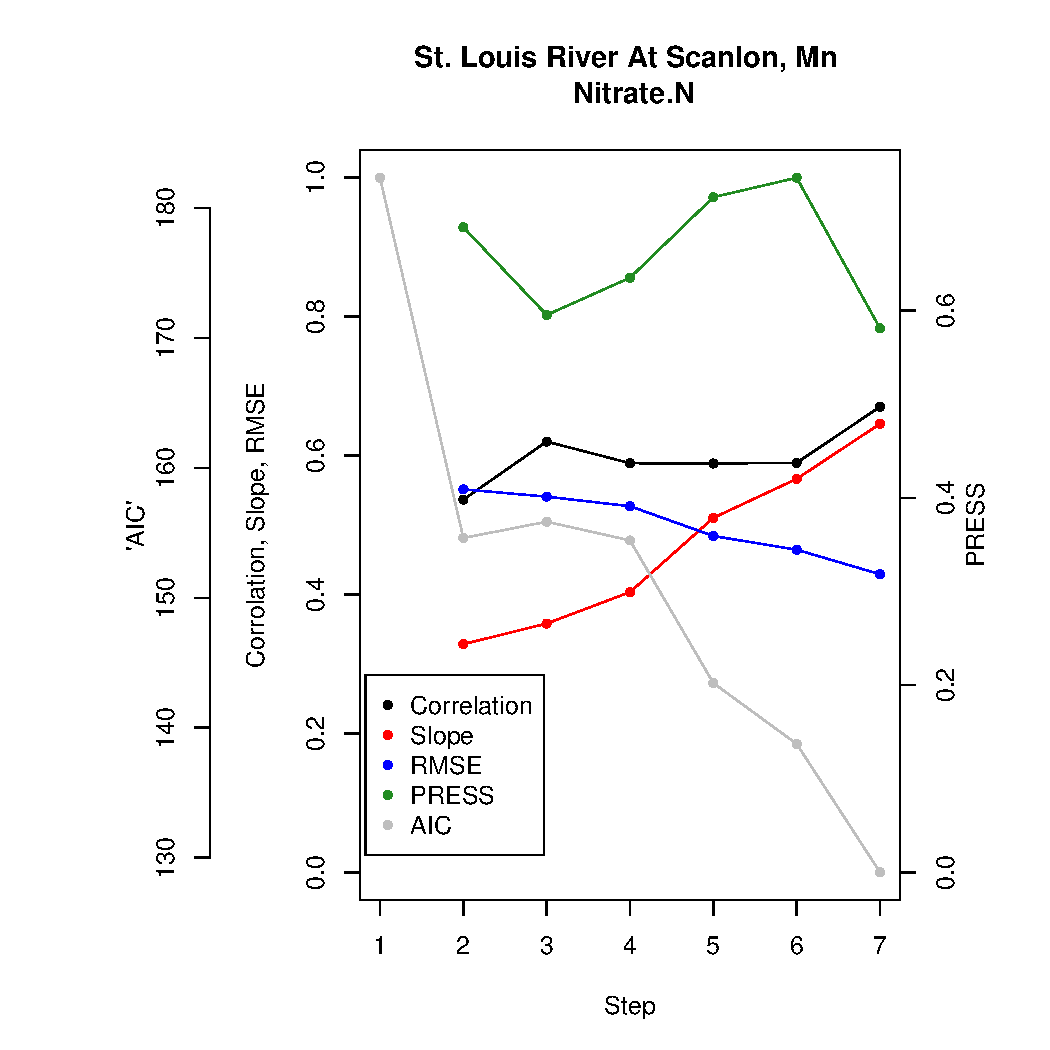
\includegraphics[width=\maxwidth]{figure/analyzeSteps} \caption[analyzeSteps]{analyzeSteps\label{fig:analyzeSteps}}
\end{figure}


\end{knitrout}

In this case, it may seem strange that the AIC value goes up then down. This is because the first parameter that was picked was sinDY (sine of decimal year). As mentioned earlier, if sinDY is picked, we automatically force cosine to be the next parameter. 

\FloatBarrier

plotSteps shows the observed versus predicted for each step along the way of the stepwise regression.There are two lines included, the blue line is a one-to-one line, the red line is the slope of the observed versus predicted values as calculated with a linear regression (lm). In this simple regression, censored values are taken as their detection limits. Red points indicate potential outliers as calculated based on external studentized residuals greater than 3 or less than -3. Censored values are represented with a line segment from the detection limit to zero (for left-censored data).


\begin{knitrout}
\definecolor{shadecolor}{rgb}{0.969, 0.969, 0.969}\color{fgcolor}\begin{kframe}
\begin{alltt}
\hlstd{m} \hlkwb{<-} \hlkwd{t}\hlstd{(}\hlkwd{matrix}\hlstd{(}\hlkwd{c}\hlstd{(}\hlnum{1}\hlopt{:}\hlnum{6}\hlstd{),} \hlkwc{nrow} \hlstd{=} \hlnum{2}\hlstd{,} \hlkwc{ncol} \hlstd{=} \hlnum{3}\hlstd{))}
\hlkwd{layout}\hlstd{(m)}
\hlkwd{par}\hlstd{(}\hlkwc{mar}\hlstd{=}\hlkwd{c}\hlstd{(}\hlnum{2}\hlstd{,}\hlnum{2}\hlstd{,}\hlnum{2}\hlstd{,}\hlnum{2}\hlstd{))}
\hlkwd{plotSteps}\hlstd{(steps,DT,transformResponse)}
\end{alltt}
\begin{verbatim}
Nitrate.N ~  sinDY 
Nitrate.N ~  sinDY + cosDY 
Nitrate.N ~  sinDY + cosDY + pH 
Nitrate.N ~  sinDY + cosDY + pH + log(SpecCond) 
Nitrate.N ~  sinDY + cosDY + pH + log(SpecCond) + Wtemp 
Nitrate.N ~  sinDY + cosDY + pH + log(SpecCond) + Wtemp + log(Turb) 
\end{verbatim}
\end{kframe}\begin{figure}[]

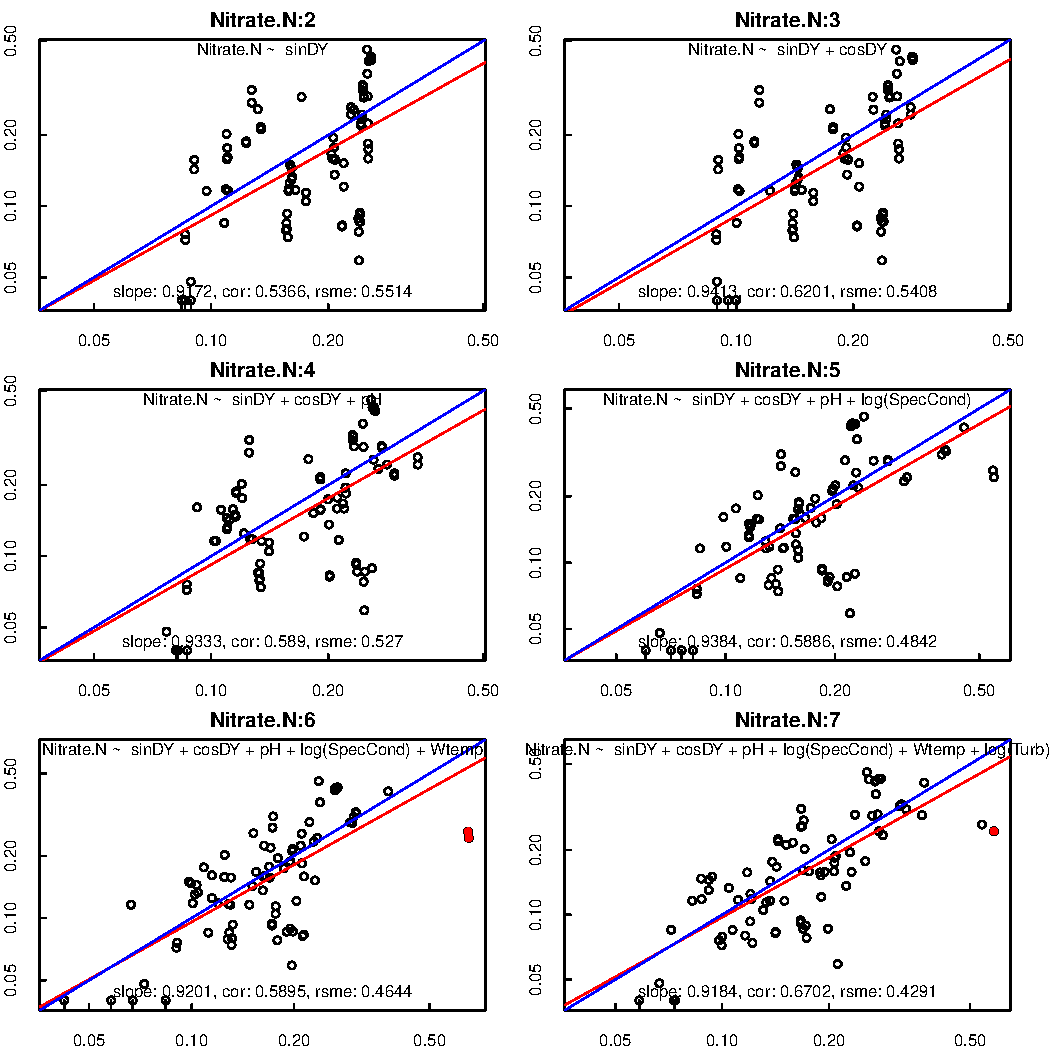
\includegraphics[width=\maxwidth]{figure/plotSteps} \caption[plotSteps]{plotSteps\label{fig:plotSteps}}
\end{figure}


\end{knitrout}

\FloatBarrier

%------------------------------------------------------------
\subsection{Model Adjustments}
%------------------------------------------------------------
There may be situations in which the user wants to explore alternative models compared to the results of the stepwise regression. The first tool offered in the package for this type of work is the function generateParamChoices. This function will create a dataframe, and optionally save it to a csv file with all of the parameter choices.

\begin{knitrout}
\definecolor{shadecolor}{rgb}{0.969, 0.969, 0.969}\color{fgcolor}\begin{kframe}
\begin{alltt}
\hlcom{#Change this to a relavent path:}
\hlstd{pathToSave} \hlkwb{<-} \hlstr{"C:/RData/"}
\hlstd{choices} \hlkwb{<-} \hlkwd{generateParamChoices}\hlstd{(predictionVariables,}
                                \hlstd{modelReturn,pathToSave,}\hlkwc{save}\hlstd{=}\hlnum{TRUE}\hlstd{)}
\end{alltt}
\end{kframe}
\end{knitrout}



This produces a file that can be opened in Microsoft Excel, or any text editor:

\begin{figure}[ht!]
\centering
 \resizebox{0.9\textwidth}{!}{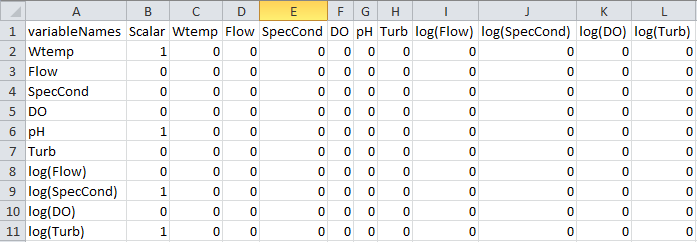
\includegraphics{Excel.png}} 
\caption{Output of generateParamChoices shown in Excel}
\label{overflow}
\end{figure}

The first column, `Scalar', is pre-populated with zeros and ones, where ones represent the variables picked in the stepwise regression. Changing the 1's and 0's in this column will allow the user to easily set which parameters should be modeled. So, adding a 1 to the Flow row in the Scalar column will tell the program to include Flow in the model (as well as any other parameters with 1's). The next set of columns are used to allow users to include interaction terms. For example, if the interaction between log(Flow) and Turbidity was thought to be useful, a 1 in row 8, column H (log(Flow):Turb) would be required.

Once the parameter choice file is adjusted, it can be read in using read.csv, and a new formula can be created using the createFormulaFromDF function.

\begin{knitrout}
\definecolor{shadecolor}{rgb}{0.969, 0.969, 0.969}\color{fgcolor}\begin{kframe}
\begin{alltt}
\hlstd{choicesNew} \hlkwb{<-} \hlkwd{read.csv}\hlstd{(pathToSave)}
\hlstd{newFormula} \hlkwb{<-}\hlkwd{createFormulaFromDF}\hlstd{(choicesNew)}
\end{alltt}
\end{kframe}
\end{knitrout}



\begin{knitrout}
\definecolor{shadecolor}{rgb}{0.969, 0.969, 0.969}\color{fgcolor}\begin{kframe}
\begin{alltt}
\hlstd{newFormula}
\end{alltt}
\begin{verbatim}
[1] "Wtemp + Flow + pH + log(SpecCond) + log(Turb) + Turb:log(Flow)"
\end{verbatim}
\end{kframe}
\end{knitrout}

From this formula, the stepwise regression routine can be re-run (if certain parameters were deleted for example), or the model can be created:

\begin{knitrout}
\definecolor{shadecolor}{rgb}{0.969, 0.969, 0.969}\color{fgcolor}\begin{kframe}
\begin{alltt}
\hlstd{newUpperFormula} \hlkwb{<-} \hlkwd{paste}\hlstd{(investigateResponse,}\hlstr{" ~ "}\hlstd{, newFormula,} \hlkwc{sep}\hlstd{=}\hlstr{""}\hlstd{)}
\hlstd{modelReturnCustom} \hlkwb{<-} \hlkwd{censReg}\hlstd{(newUpperFormula,}
                       \hlkwc{dist}\hlstd{=transformResponse,} \hlkwc{data}\hlstd{=DT)}
\hlstd{modelReturnCustom}
\end{alltt}
\begin{verbatim}
Call:
censReg(formula = Nitrate.N ~ Wtemp + Flow + pH + log(SpecCond) + 
    log(Turb) + Turb:log(Flow), data = DT, dist = transformResponse)

Coefficients:
                 Estimate Std. Error  z-score p-value
(Intercept)     7.879e+00  2.538e+00  3.10485  0.0017
Wtemp          -3.029e-02  7.959e-03 -3.80579  0.0002
Flow           -4.829e-05  3.452e-05 -1.39901  0.1440
pH             -1.131e+00  3.494e-01 -3.23676  0.0011
log(SpecCond)  -1.023e-01  4.238e-01 -0.24147  0.7980
log(Turb)      -1.343e-02  1.416e-01 -0.09488  0.9235
Turb:log(Flow)  7.178e-04  1.385e-03  0.51844  0.5872

Estimated residual standard error (Unbiased) = 0.574
Distribution: lognormal
Percent standard error: 62.47
Positive percent error: 77.54
Negative percent error: -43.68

Number of observations = 85, number censored = 5 (5.9 percent)

Loglik(model) = -72.23 Loglik(intercept only) = -86.72
  Chi-square = 28.98, degrees of freedom = 6, p-value = <0.0001

Computation method: AMLE
\end{verbatim}
\end{kframe}
\end{knitrout}

%------------------------------------------------------------
\subsection{Model Analysis}
%------------------------------------------------------------
Finally, the package offers several ways to analyze and report on the model results. We will look at the results of the original model returned from the stepwise regression (not the custom model we created in the last section). Censored values are plotted as points with segments (from the detection limit towards zero for left-censored data). Also, left-censored residuals are calculated using the detection limit.

The function resultPlots plots a set of plots. All model results include observed vs. predicted (A), residuals vs. predicted (B), residuals vs. time (C), and residual quantiles vs. theoretical quantiles (D). After that, there is a plot for observed vs. each parameter in the model (E...).

\begin{knitrout}
\definecolor{shadecolor}{rgb}{0.969, 0.969, 0.969}\color{fgcolor}\begin{kframe}
\begin{alltt}
\hlkwd{resultPlots}\hlstd{(DT,modelReturn,siteINFO)}
\end{alltt}
\end{kframe}\begin{figure}[]

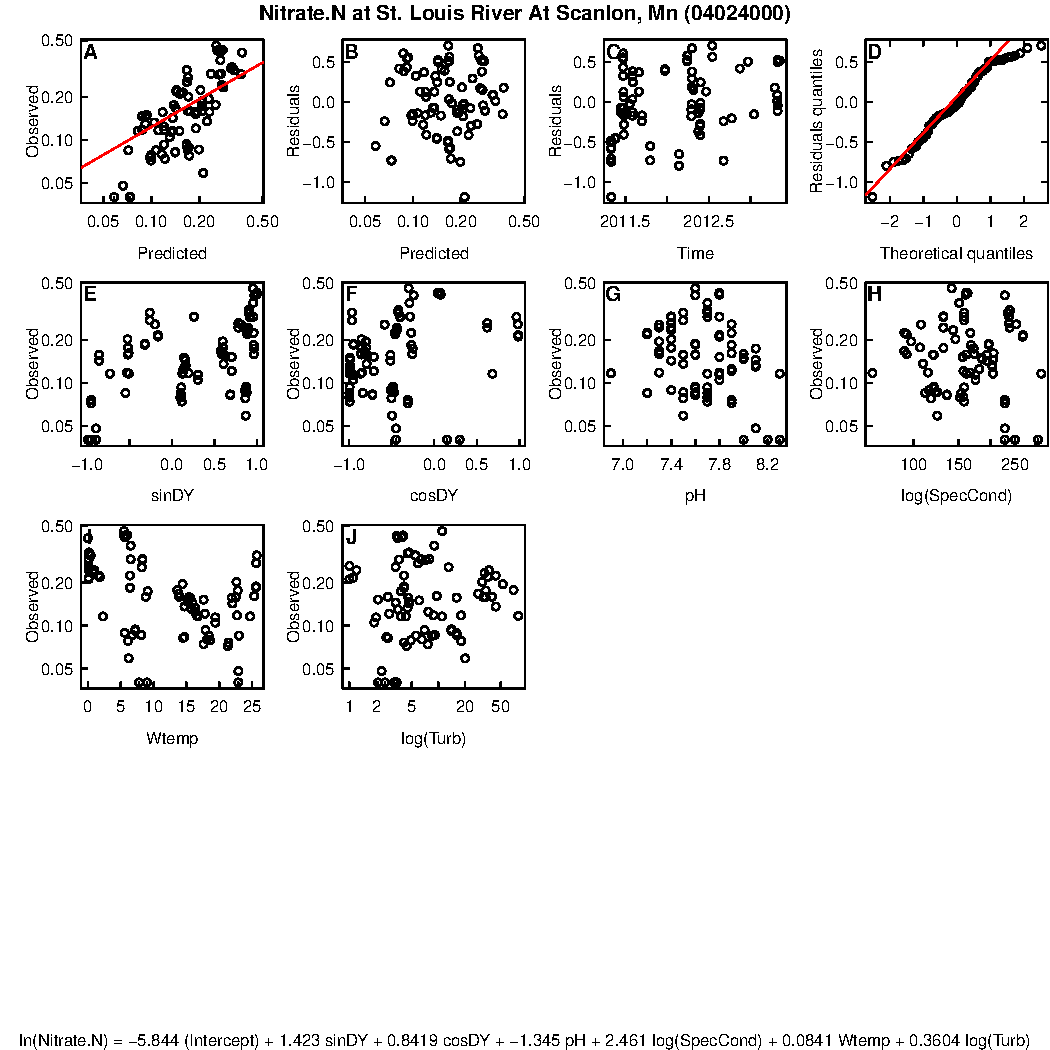
\includegraphics[width=\maxwidth]{figure/resultPlots} \caption[resultPlots]{resultPlots\label{fig:resultPlots}}
\end{figure}


\end{knitrout}

\FloatBarrier

The function resultResidPlots plots a set of plots. All model results include observed vs. predicted (A), residuals vs. predicted (B), residuals vs. time (C), and residual quantiles vs. theoretical quantiles (D). After that, there is a plot for residuals vs. each parameter in the model (E...).


\begin{knitrout}
\definecolor{shadecolor}{rgb}{0.969, 0.969, 0.969}\color{fgcolor}\begin{kframe}
\begin{alltt}
\hlkwd{resultResidPlots}\hlstd{(DT,modelReturn,siteINFO)}
\end{alltt}
\end{kframe}\begin{figure}[]

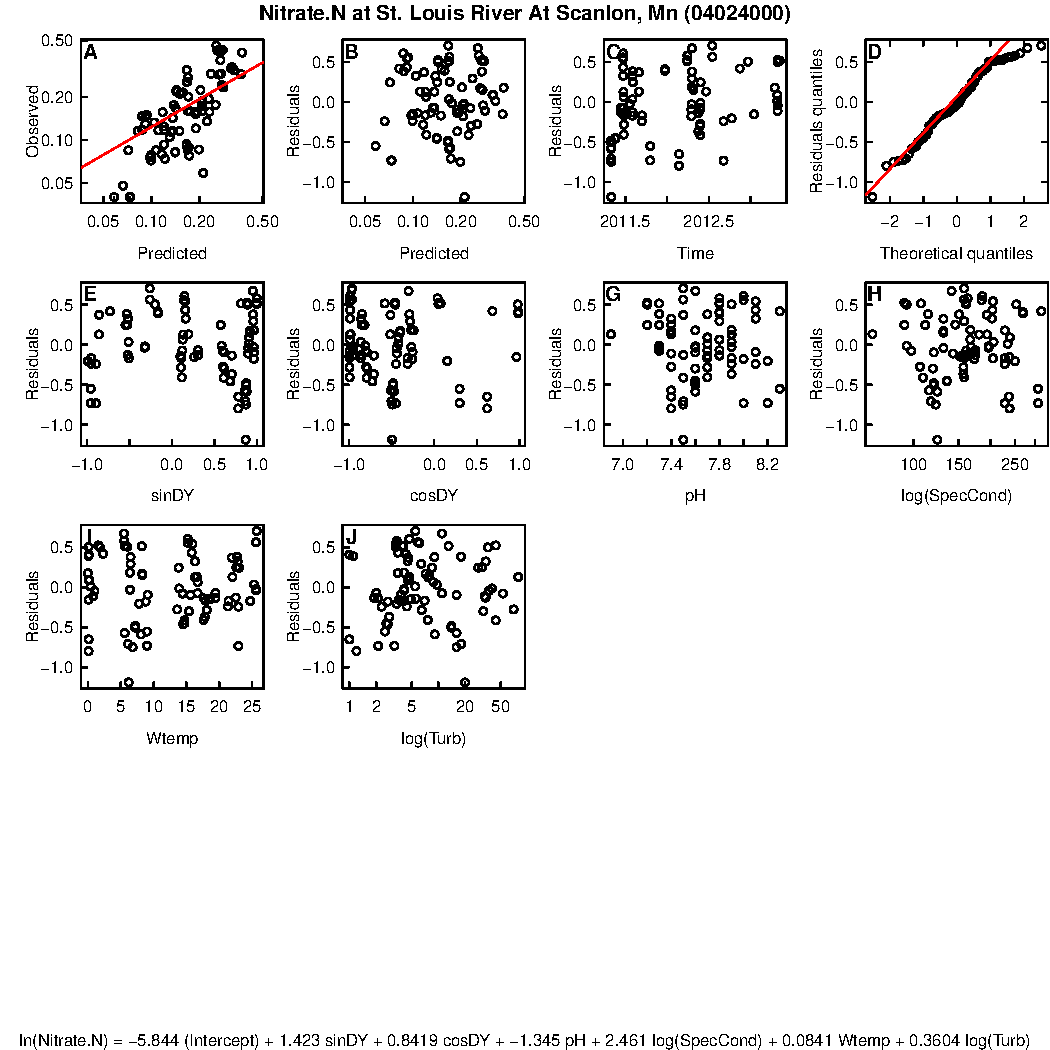
\includegraphics[width=\maxwidth]{figure/resultResidPlots} \caption[resultResidPlots]{resultResidPlots\label{fig:resultResidPlots}}
\end{figure}


\end{knitrout}

\FloatBarrier

The predictionPlot function plots the predicted values based on all of the unit value data available (from the UV dataframe) in blue. Red dots representing the actual measured data are also included. Left-censored points are shown at their detetction limit, with a segment going towards zero.


\begin{knitrout}
\definecolor{shadecolor}{rgb}{0.969, 0.969, 0.969}\color{fgcolor}\begin{kframe}
\begin{alltt}
\hlkwd{predictionPlot}\hlstd{(UV,DT,modelReturn,}\hlkwc{siteINFO}\hlstd{=siteINFO)}
\end{alltt}
\end{kframe}\begin{figure}[]

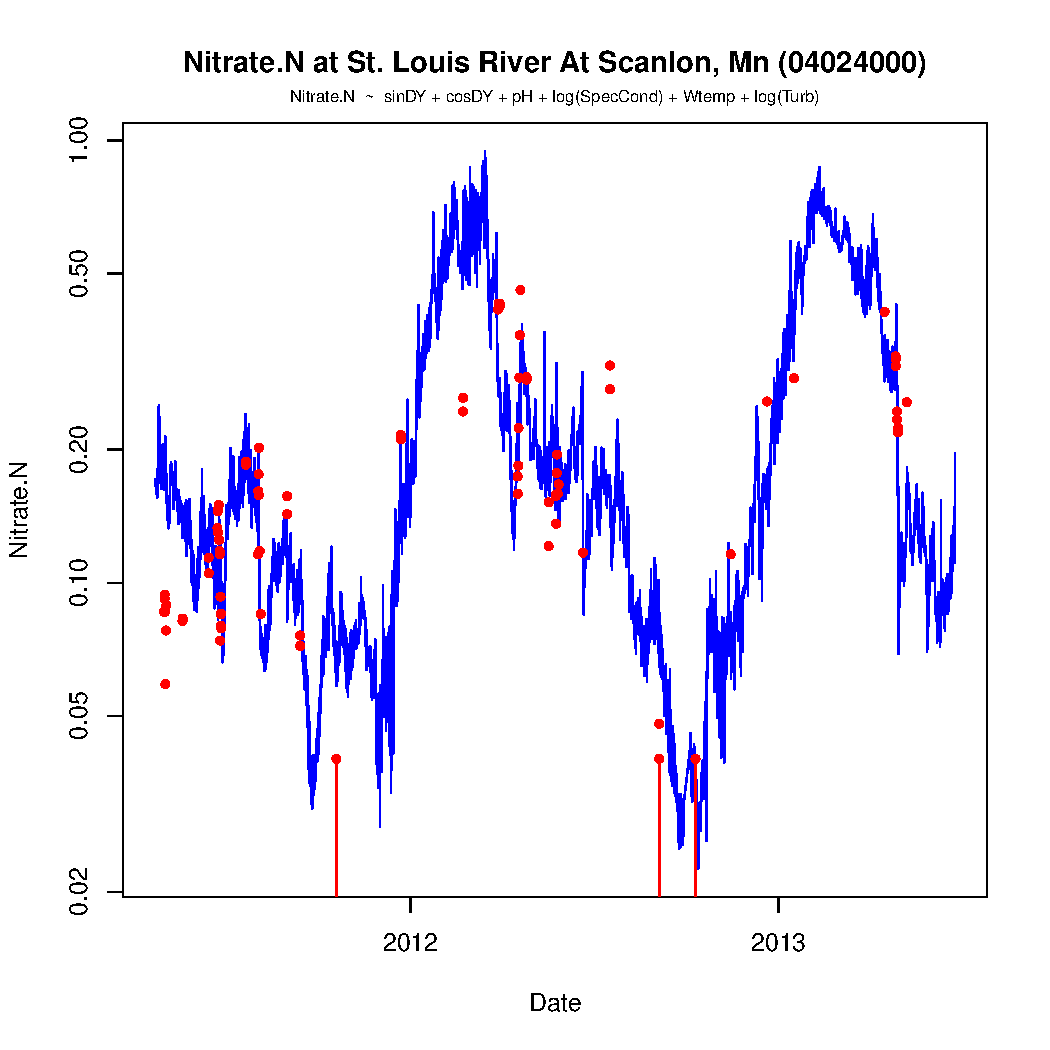
\includegraphics[width=\maxwidth]{figure/predictionPlot} \caption[predictionPlot]{predictionPlot\label{fig:predictionPlot}}
\end{figure}


\end{knitrout}

\FloatBarrier
Finally, a summary printout can be obtained with the function summaryPrintout in either the R console or saved to a file.

\begin{knitrout}
\definecolor{shadecolor}{rgb}{0.969, 0.969, 0.969}\color{fgcolor}\begin{kframe}
\begin{alltt}
\hlkwd{summaryPrintout}\hlstd{(modelReturn, siteINFO)}
\end{alltt}
\begin{verbatim}
Nitrate.N  at  St. Louis River At Scanlon, Mn  ( 04024000 )
Number of observations:  85 
Distribution:  lognormal 
Method:  AMLE 
Degrees of freedom:  14 
RMSE:  0.4291 
RSQ:  61.53 
Number of censored values:  5 
Nitrate.N ~ (Intercept) + sinDY + cosDY + pH + log(SpecCond) + Wtemp + log(Turb) 

           Term Coefficient StdError pValue StCoef
1   (Intercept)      -5.844    2.336   0.01 -2.502
2         sinDY       1.423    0.178   0.00  8.002
3         cosDY       0.842    0.211   0.00  3.996
4            pH      -1.345    0.264   0.00 -5.099
5 log(SpecCond)       2.461    0.405   0.00  6.074
6         Wtemp       0.084    0.018   0.00  4.768
7     log(Turb)       0.360    0.095   0.00  3.774
8      logSigma       0.184    0.028   0.00  6.481

Correlation matrix of coefficients: 
              (Intercept)   sinDY   cosDY      pH
(Intercept)        1.0000 -0.6214 -0.3342 -0.4422
sinDY             -0.6214  1.0000  0.6207 -0.0938
cosDY             -0.3342  0.6207  1.0000  0.1125
pH                -0.4422 -0.0938  0.1125  1.0000
log(SpecCond)     -0.5749  0.6560  0.1692 -0.4760
Wtemp             -0.5114  0.8580  0.8391 -0.0300
log(Turb)         -0.7868  0.6155  0.4931  0.0740
logSigma          -0.0059  0.0376  0.0142 -0.0228
              log(SpecCond)   Wtemp log(Turb) logSigma
(Intercept)         -0.5749 -0.5114   -0.7868  -0.0059
sinDY                0.6560  0.8580    0.6155   0.0376
cosDY                0.1692  0.8391    0.4931   0.0142
pH                  -0.4760 -0.0300    0.0740  -0.0228
log(SpecCond)        1.0000  0.4712    0.6765   0.0242
Wtemp                0.4712  1.0000    0.5820   0.0283
log(Turb)            0.6765  0.5820    1.0000   0.0144
logSigma             0.0242  0.0283    0.0144   1.0000
\end{verbatim}
\end{kframe}
\end{knitrout}

\clearpage
\appendix

%------------------------------------------------------------ 
\section{Getting Started in R}
\label{sec:appendix1}
%------------------------------------------------------------ 
This section describes the options for downloading and installing the GSqwsr package.

%------------------------------------------------------------
\subsection{New to R?}
%------------------------------------------------------------ 
If you are new to R, you will need to first install the latest version of R, which can be found here: \url{http://www.r-project.org/}.

There are many options for running and editing R code, one nice environment to learn R is RStudio. RStudio can be downloaded here: \url{http://rstudio.org/}. Once R and RStudio are installed, the dataRetrieval package needs to be installed as described in the next section.

At any time, you can get information about any function in R by typing a question mark before the functions name.  This will open a file (in RStudio, in the Help window) that describes the function, the required arguments, and provides working examples.

\begin{knitrout}
\definecolor{shadecolor}{rgb}{0.969, 0.969, 0.969}\color{fgcolor}\begin{kframe}
\begin{alltt}
\hlkwd{library}\hlstd{(GSqwsr)}
\hlopt{?}\hlstd{plotSteps}
\end{alltt}
\end{kframe}
\end{knitrout}

To see the raw code for a particular code, type the name of the function:
\begin{knitrout}
\definecolor{shadecolor}{rgb}{0.969, 0.969, 0.969}\color{fgcolor}\begin{kframe}
\begin{alltt}
\hlstd{plotSteps}
\end{alltt}
\end{kframe}
\end{knitrout}

%------------------------------------------------------------
\subsection{R User: Installing QWSR}
%------------------------------------------------------------ 
Before installing GSqwsr, the dependent packages must be first be installed:

\begin{knitrout}
\definecolor{shadecolor}{rgb}{0.969, 0.969, 0.969}\color{fgcolor}\begin{kframe}
\begin{alltt}
\hlkwd{install.packages}\hlstd{(}\hlkwd{c}\hlstd{(}\hlstr{"USGSwsBase"}\hlstd{,}\hlstr{"USGSwsStats"}\hlstd{,}
                   \hlstr{"USGSwsData"}\hlstd{,}\hlstr{"USGSwsGraphs"}\hlstd{,}
                   \hlstr{"USGSwsQW"}\hlstd{,}\hlstr{"dataRetrieval"}\hlstd{,}\hlstr{"GSqwsr"}\hlstd{),}
      \hlkwc{repos}\hlstd{=}\hlkwd{c}\hlstd{(}\hlstr{"http://usgs-r.github.com"}\hlstd{,}\hlstr{"http://cran.us.r-project.org"}\hlstd{),}
      \hlkwc{dependencies}\hlstd{=}\hlnum{TRUE}\hlstd{)}
\end{alltt}
\end{kframe}
\end{knitrout}


After installing the package, you need to open the library each time you re-start R.  This is done with the simple command:
\begin{knitrout}
\definecolor{shadecolor}{rgb}{0.969, 0.969, 0.969}\color{fgcolor}\begin{kframe}
\begin{alltt}
\hlkwd{library}\hlstd{(GSqwsr)}
\end{alltt}
\end{kframe}
\end{knitrout}




\end{document}
